%%% template.tex
%%%
%%% This LaTeX source document can be used as the basis for your technical
%%% paper or abstract. Regardless of the length of your document, the commands
%%% are all the same.
%%% 
%%% The "\documentclass" command is the first command in your file. If you want to 
%%% prepare a version of your article with line numbers - a "review" version - 
%%% include the "review" parameter:
%%%    \documentclass[review]{acmsiggraph}
%%%


\documentclass{acmsiggraph}

%%%packages to include
\usepackage{todonotes}
%%% Title of your article or abstract.

\title{Fused AR Experience}

\author{David~Dunn\thanks{e-mail:dunn@unc.edu}\\Abdul~Rafay~Khalid\thanks{e-mail:arkhalid@cs.unc.edu}} 
\pdfauthor{Abdul~Rafay~Khalid}

%%% Used by the ``review'' variation; the online ID will be printed on 
%%% every page of the content.

\TOGonlineid{45678}

% User-generated keywords.

\keywords{KinectFusion, RGBD, Augmented Reality}

% With the "\setcopyright" command the appropriate rights management text will be added
% to your document.

%\setcopyright{none}
%\setcopyright{acmcopyright}
%\setcopyright{acmlicensed}
\setcopyright{rightsretained}
%\setcopyright{usgov}
%\setcopyright{usgovmixed}
%\setcopyright{cagov}
%\setcopyright{cagovmixed}
%\setcopyright{rightsretained}

% The year of publication in the "\copyrightyear" command.

\copyrightyear{2016}

%%% Conference information, from the completed rights management form.
%%% The "\conferenceinfo" command has two parameters: 
%%%    - conference name
%%%    - conference date and location
%%% The "\isbn" field includes the year and month after the article ISBN.

\conferenceinfo{SIGGRAPH 2016 Posters}{July 24-28, 2016, Anaheim, CA} 
\isbn{978-1-4503-ABCD-E/16/07} 
\doi{http://doi.acm.org/10.1145/9999997.9999999}

\begin{document}

%%% This is the ``teaser'' command, which puts an figure, centered, below 
%%% the title and author information, and above the body of the content.

 \teaser{
   \includegraphics[height=1.5in]{images/sampleteaser}
   \caption{Spring Training 2009, Peoria, AZ.}
 }

\maketitle

\begin{abstract}
Traditionally Augmented Reality has taken three main forms each with its own drawbacks. Optical see-through gives us a good view of the real world but it is difficult to show virtual objects effectively as occlusion cannot be achieved. Spatial Augmented reality doesn't allow the user to view the virtual content at the correct depth. The closest to approach to ours is Video See through augmented reality however it suffers from mismatch between the location of eye and the camera center. In recent years there has been a lot of work on accurately reconstructing a 3D representation of the environment using RGBD sensors. We propose a system that combines such a realtime reconstruction method with a Head mounted display to create a wide field of view Augmnented Reality system. 

\end{abstract}

%
% The code below should be generated by the tool at
% http://dl.acm.org/ccs.cfm
% Please copy and paste the code instead of the example below. 
%
\begin{CCSXML}
<ccs2012>
<concept>
<concept_id>10010147.10010371.10010382</concept_id>
<concept_desc>Computing methodologies~Image manipulation</concept_desc>
<concept_significance>500</concept_significance>
</concept>
<concept>
<concept_id>10010147.10010371.10010382.10010236</concept_id>
<concept_desc>Computing methodologies~Computational photography</concept_desc>
<concept_significance>300</concept_significance>
</concept>
</ccs2012>
\end{CCSXML}

\ccsdesc[500]{Computing methodologies~Image manipulation}
\ccsdesc[300]{Computing methodologies~Computational photography}

%
% End generated code
%

% The next three commands are required, and insert the user-generated keywords, 
% The CCS concepts list, and the rights management text.
% Please make sure there is a blank line between each of these three commands.

\keywordlist

\conceptlist

\printcopyright

\section{Introduction}


Recent advances in reconstruction methods means that we can create a 3D representation of an environment in real time. The ability of these methods lead us to imagine an alternate form of Augmented Reality. By attaching an RGBD sensor to a VR HMD we can reconstruct the environment around the user as he moves around in his environment. As we have a 3D model of the environment we can render the view from each of the user's eyes. This enables us to accurately reproduce the real environment of the user in stereo. Virtual content can then be composited over the model of the real environment. By using the tracking from the reconstruction method we can align the virtual content with the reconstruction. 

\begin{figure}[ht]
	\centering
	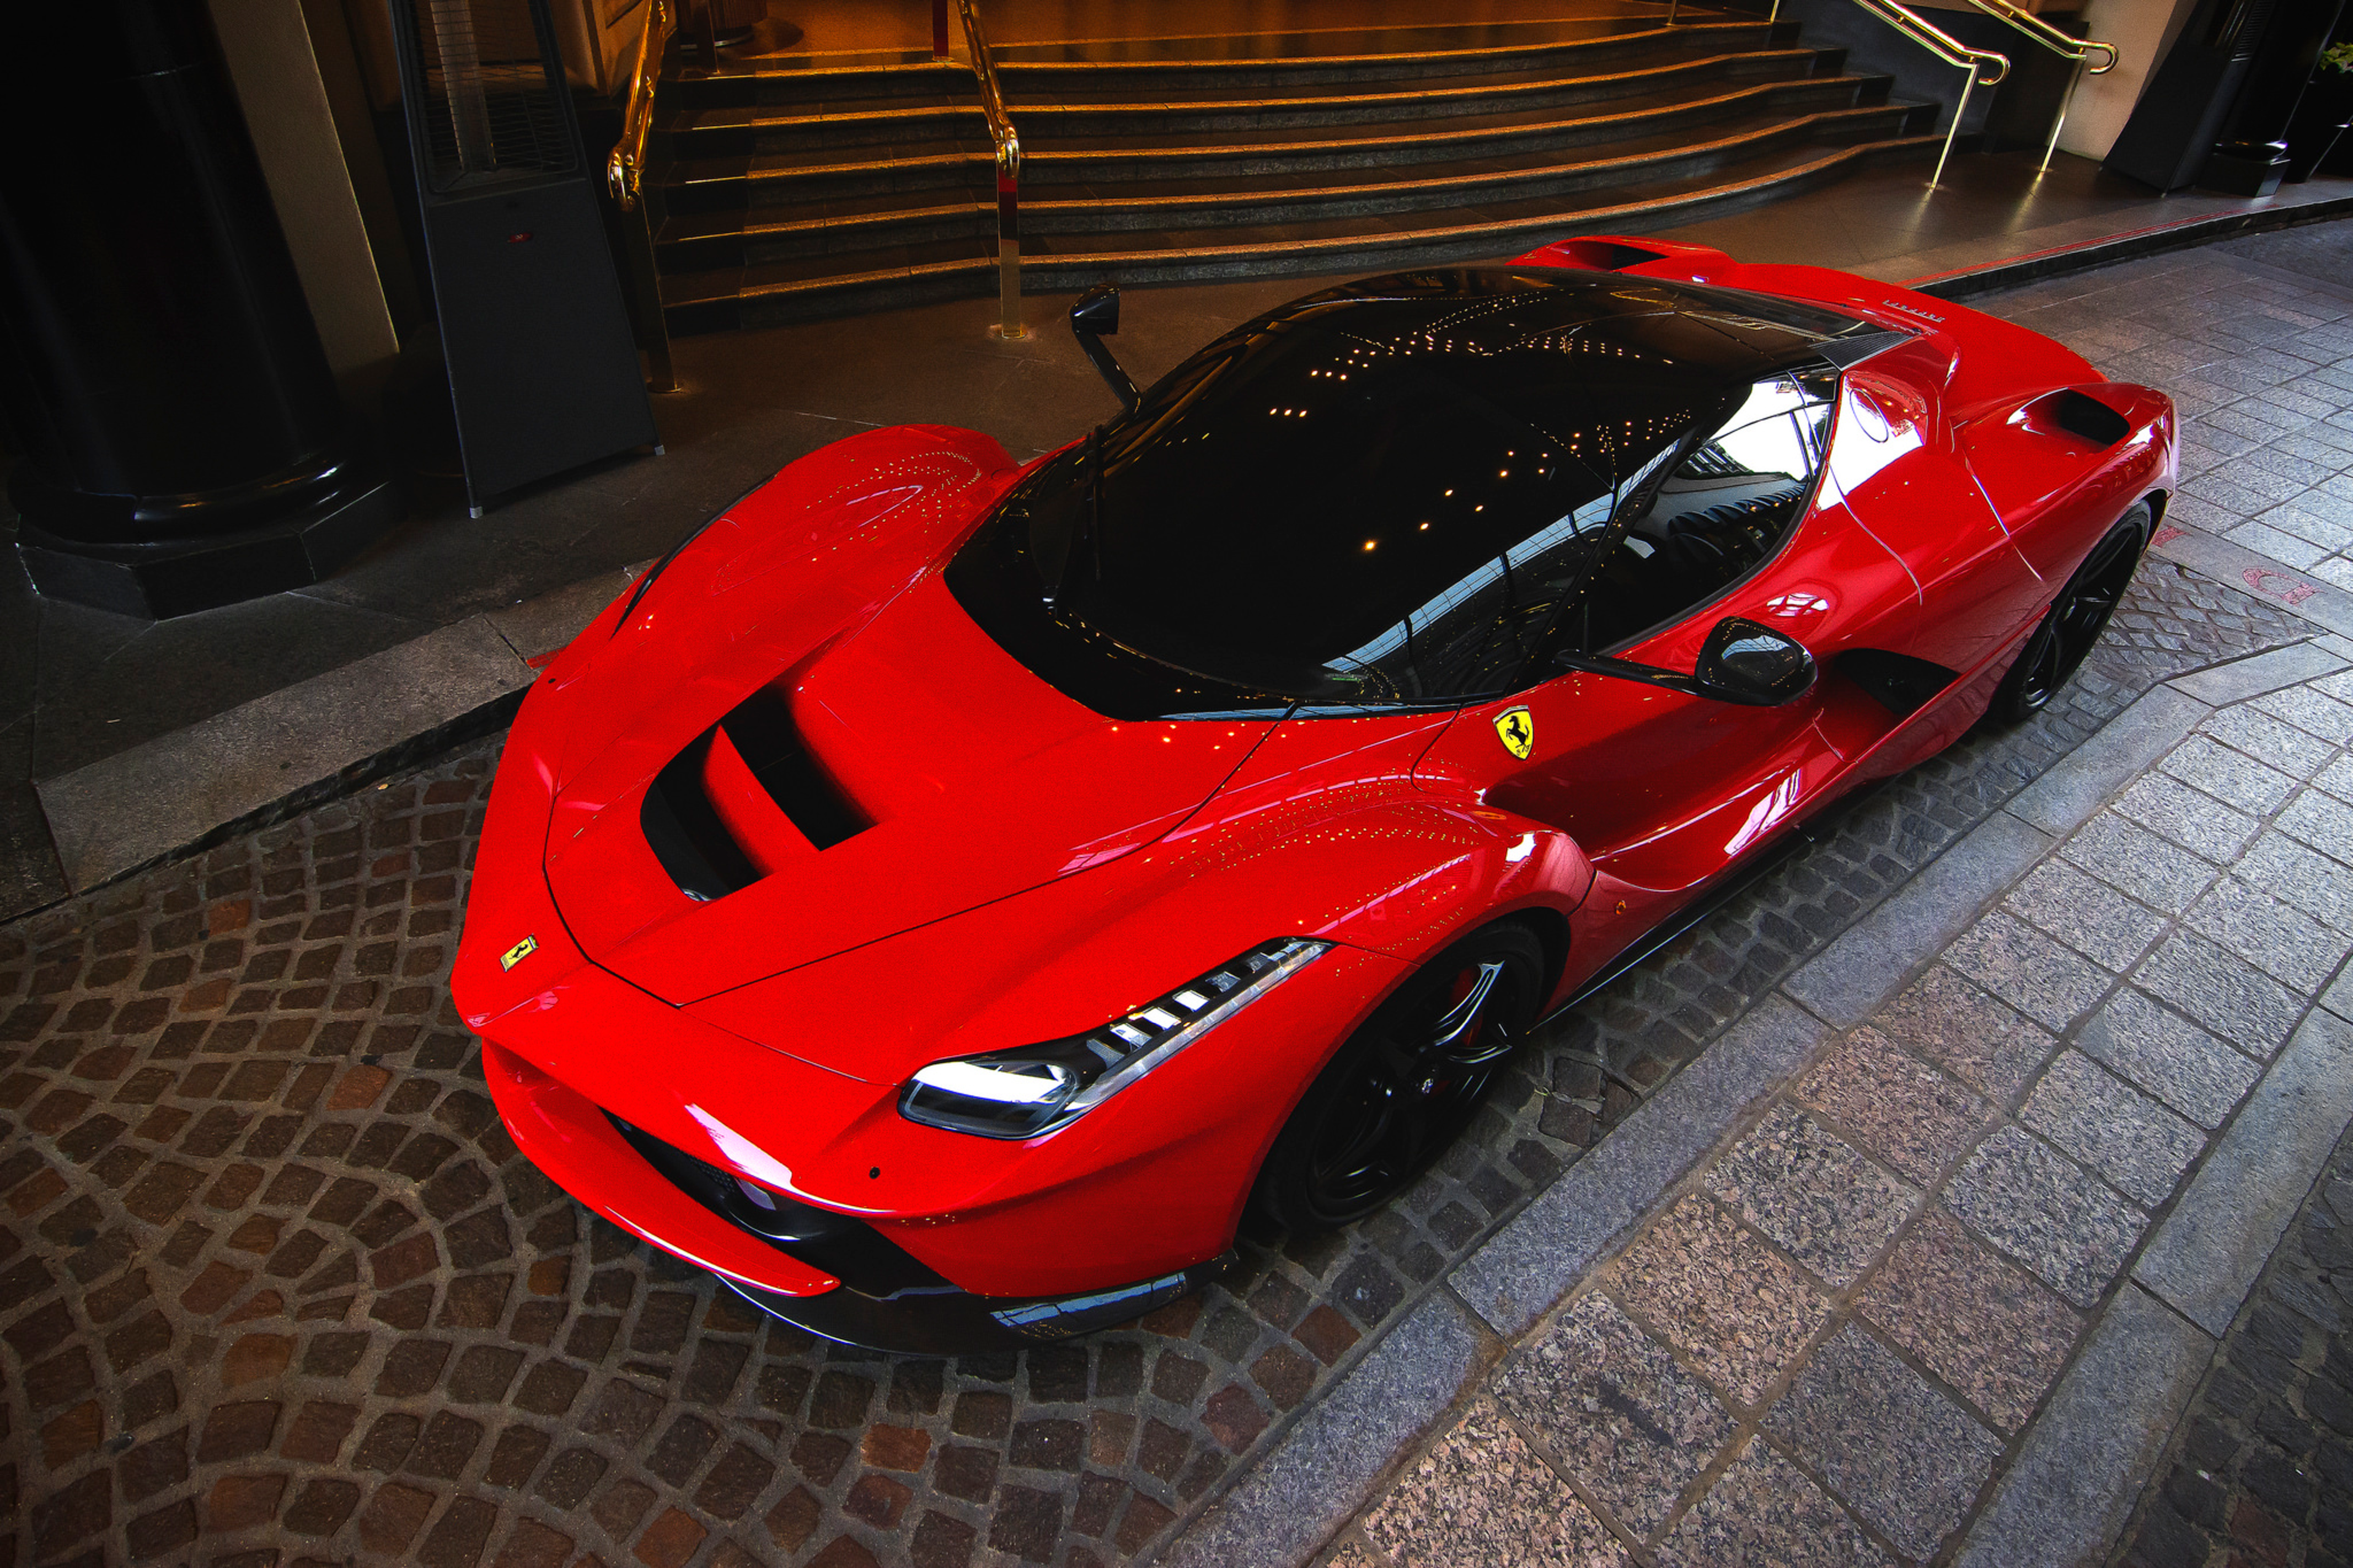
\includegraphics[width=3.0in]{images/ferrari_laferrari}
	\caption{Ferrari LaFerrari. Image courtesy Flickr user ``gfreeman23.''}
	\label{fig:ferrari}
\end{figure}
\section{Related Work}





\section{System Design}
Our setup consists of a Kinect camera rigidly aligned to an Oculus Rift HMD (Figure  \todo[inline]{Add picture of rft and kinect} ). The kinect acquires RGBD images which as used as input to the KinectFusion algorithm. Using the RGBD images, KinectFusion estimates the camera pose and uses this to integrate the current depthmap into the reconstruction. Virtual content is generated by animating a rigged model of a virtual character. The reconstruction is rendered from the viewpoint of the eyes. The virtual content is then composited onto this. If the virtual content is transformed using the same tracking as the reconstruction then it remains aligned to the environment.The combination of the reconstruction and virtual content is then rendered onto the HMD. Figure \todo[inline]{Add system overview figure} shows the System Overview. 
\missingfigure{System Overview}

\missingfigure{Picture of Rift}


\subsection{Environment Capture}
In order to capture the environment, we rely on the KinectFusion\cite{newcombe2011kinectfusion}  algorithm as our environment is static and we require the algorithm to be realtime. There are two main implementations of KinectFusion available. The Kinect Development Toolkit for Windows comes with an API to access KinectFusion. They do not provide source code but let the developer access KinectFusion in a limited matter. Also this version has only been demonstrated on small volumes and the tracking is not very stable when using large volumes with small voxel denisty. Given a camera pose and a camera matrix, the API allows the user to render the scene from that camera.\\
The other popular implementation is the one that comes with PCL. This contains extensions on KinectFusion that enable it to work in large areas. It does so by decomposing the environment into chunks that can be uploaded to the GPU. This allows it to reconstruct a large volume while maintaining a high voxel density.This results in more robust tracking.  


\subsection{Generate Virtual Content}

Creating virtual content has been at the foundations of computer graphics since its inception. Many processes have been developed over the years to solve the problem. Our aim was to create a digital character (dragon) which could fly around the real environment. Due mostly to our background in the movie industry, we have chosen a workflow designed for digital artists and facilitated by commercial software, namely Autodesk Maya. The process consists of the following steps:

\begin{enumerate}
	\item Modeling 
	\item Texturing or Look-Development
	\item Rigging or Character Setup
	\item Animating
\end{enumerate}

Each of these steps consists of an additive process where elements are added upon the output of the previous step and are pushed further down the chain. Typical workflows are designed such that for as many steps as possible, modifications will be non-destructive to steps further down the chain.

Modeling can be likened to digital sculpture; the primary goal being the creation of a mesh, usually polygonal, that represents the object being created. The two dimensional polygons represent the outer surface of the object or character and are connected in complex patterns to create a three dimensional structure approximating the surface of the object. The exact layout of the polygons does not matter for the look of the object, however considerations must be made for the steps further down the pipeline. Texturing becomes more difficult if large polygons are connected to small polygons, so even distribution is sought after, while rigging becomes more difficult if the edges of the polygonal faces do not align with the axis of movement, so typically quadrilateral polygons are chosen. The output of modeling is a mesh.

Texturing and look-development can be likened to painting a sculpture; it is primarily concerned with the look of the surface that was created by modeling. This is achieved through various means of defining the color generated by the mesh when it is rendered. This can be achieved both by manipulating the texture of the object and by changing the shader it is rendered with. Textures are similar to wallpaper or gift wrap: it spreads a flat image across the surface of a polygon shape either by use of UVs\cite{catmull1974subdivision} or a more complex process such as Ptex. Shading defines how the surface is shown when rendered and typically involves manipulating light from multiple sources to create a color. The output of texturing and look-development is a textured and shaded mesh. 

Rigging or character setup is like taking a sculpture or statue and turning it into a puppet; it is the process of adding the capability of motion to the mesh. While many different means of creating motion exist, the simplest involves three steps: adding bones or joints, adding controls to manipulate the joints, and binding the joints to the mesh with a deformer. Joints consists of hierarchical transforms which can easily be transformed to create complex motion. They can be likened to the bones inside any animal. Controls are the means by which the animator will move the joints in complex ways. Accommodating the needs of the animator should be of utmost consideration - simple controls that are intuitive but give complete control are the goal. To this end tools such as inverse kinematics (IK), forward kinematics (FK), and space switching are employed. In order to let the joints drive the mesh, a deformer, which encodes a complex series of mappings from joints to vertices on the mesh, is used. The process of creating and altering the mappings is called skinning and the key consideration is creating natural looking motions which are both smooth and volume preserving. The output of rigging is a character rig.

Animating is the process of creating motion over time. The character rig is posed using the controls that were set up and keys are set on a particular frame such that the attributes which are keyed will evaluate to the set value when given the frame. Just as in any continuous function, the values between keys are interpolated. The method of interpolation can be controlled so that the desired motion is achieved. The output of animation is a mesh moving through time.

\subsubsection{A Dragon Comes to Life}
In following the traditional animation pipeline, we determined that we did not have enough time and it was outside of our scope to create an entire character from scratch, so we sought out a character model online. Of all the dragons which can be obtained for free online, only one was created with rigging in mind. It was modeled using quads and textured and even provided a rig\cite{dragon}. We proceeded to animate the dragon in a flying sequence such that it would be able to fly around the real room environment around the user.
\begin{figure}[ht]
	\centering
	\includegraphics[width=3.0in]{images/cycle.0012.png}
	\caption{A sample frame of our dragon flight animation.}
	\label{fig:dragon}
\end{figure}
As we did not use a game engine for our application, we did not have a freely built-in deformer that could manipulate our dragon mesh over time. It was also outside the scope of this project to create a deformer, so we needed a solution. Our solution was to export our animation sequence frame by frame into the .obj format, which contains both polygonal and texture data. We then would load all the frames into memory and render them in sequence. Thus it was that a dragon came to life.


\subsection{Composit Real and Virtual Content}
We use the textures from KinectFusion as background and composit it with our virtual content.

\subsection{Tracking}
KinectFusion uses the current depth image and tries to align it with the reconstruction to find out the camera pose. This camera pose is used to track the head-mount with respect to the world. The same transform needs to be applied to the virtual content to keep it fixed with respect to the real world. For our initial experiments however, the rotational tracking from the Oculus was used to align the virtual objects. This can be shifted without too much effort to use the tracking from KinectFusion ensuring that the objects stay aligned to the real world.

\subsection{Display on HMD}
To render on the HMD, we draw our content on the framebuffer provided by Oculus Rift SDK for each eye. In order to ensure that the content looks correct through the oculus, we provide the desired FOV and texture size expected by the Rift to the KinectFusion API. Some further calibration was performed to ensure that objects in the Oculus appeared the same size as the real world. In our setup, the Kinect is placed above the Rift and thus the perspective from which its looks at the environment is different than the eye. We transform the Kinect to the pose of the centre of the Rift. Eye Position translations are then applied to get the poses for the eyes. The environment is rendered from each of the poses and passed to the Rift. The additional virtual content is rendered on the same buffers. The rift applies lens distortion correction and displays it.

\section*{Acknowledgements}

To Robert, for all the bagels.

\bibliographystyle{acmsiggraph}
\nocite{*}
\bibliography{template}
\end{document}
